%This is where the state of the art goes:
%\begin{itemize}
%\item what is aggregation in a smart grid context?
%\item What is being aggregated?
%\item What is the purpose of the aggregation (delivery of which product?) 
%\item Which types of design exist (examples, not categorisation yet - we'll do that later) Examples
%\item Outcome: Why are aggregators an issue in smart grids?
%\end{itemize}
We refer to the concept of aggregation as the  creation and (commercial and technical) management of a portfolio of flexibility assets with the objective of offering the combined flexibility as a commercial service. The business role and technical function of performing aggregation is referred to as the Aggregator. In literature and business context use of these and related terms is not yet harmonized.
\begin{figure}[t!]
\centering
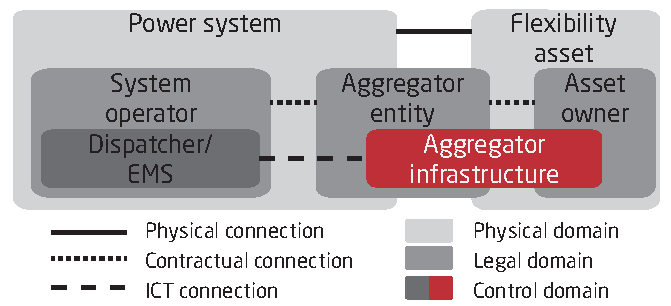
\includegraphics[width=1.0\columnwidth]{etfa2015/domains.eps}
\caption{The aggregator concept across domains.}
\label{fig:domains}
\vspace*{-5mm}
\end{figure}
\subsection{Clarifying the Aggregator concept}\label{subsec:clarifying}
The term \emph{aggregation} has different relevant interpretations in business, information technology,  control, as well as in the physical power system domain. Our concept of aggregators is illustrated in Fig.~\ref{fig:domains}, defining aggregators as a business role, aggregator entity, as well as a technical aggregator infrastructure.

The physical domain addresses the electrical interactions between flexibility assets (also referred to as DER) and power system. Whereas aggregation with respect to physical topology is a common concept (e.g. microgrids, cells), in our understanding, aggregators are not bound to aggregation with respect to physical network topology. 
%The aggregator is only reflected in this level by the manipulation of the interaction between the flexibility assets and the power system.

In the legal and business domain, an aggregator entity is an intermediary, maintaining contractual relations with flexibility asset owners and system operators (as receivers of flexibility services). The aggregator entity assumes legal responsibility for the delivery of a contracted service. The aggregator role may be filled by new independent market actors or be part of existing actors, such as utilities or balance responsible parties.

In the control domain, the aggregator infrastructure coordinates the behavior of flexibility assets. The control domain requirements are formulated as \emph{flexibility services} to system operators and \emph{asset management services} towards asset owners. Tracing these requirements for architectural validation and performance validation in the aggregator infrastructure is the focus of this paper.

The proposed aggregator concept is implementation agnostic and focused on formulation of functional requirements.

\subsection{The aggregator concept in technical literature}
There is no unanimous definition in literature of what could be considered standard functionality of an aggregator. This is reflected by the wide variety of aggregator designs\fcite{kok2005powermatcher,han2010development,sortomme2011optimal,costanzo2013coordination}, which differ in capabilities and purpose, and which use different (often implicit) criteria for classification.

Aggregators are commonly classified by control scheme into autonomous, indirect, transactional and direct control \fcite{Kosek}. Another classification emphasizes the commercial or technical focus of aggregators, referring to \emph{commercial} and \emph{technical} virtual power plants (CVPP and TVPP) \fcite{fenix2009}; however, as both types require business and technical functionality, the CVPP/TVPP distinction expresses a difference in degree and is not categorical. An advanced aggregator realizing the full functionality spectrum as \emph{Dynamic VPP} (DVPP) has been formulated in other work\fcite{niesse2014conjoint}. 
The proposed concept of aggregation encompasses all of the above but focuses on functional requirements for service provision, not business logic.

\subsection{Aggregator Business Harmonization and Standardization}
Whereas aggregator functionality is becoming a shared concept, there are still many models describing a) which stakeholders may benefit from the flexibility service, b) the form of the flexibility service, c) which stakeholders (are allowed to) perform aggregation and who should receive compensation \fcite{eurel-aggr} and d) how to harmonize the interaction between aggregators and aggregated units.

With respect to a), market models are being revised and new service models introduced to assign a value to flexibility (either directly to system operators as ancillary service, or as enhancement of flexibility of existing portfolios). The form of the service, b), is often formulated as an abstract flexibility service, a trade-off between both grid needs and generalized resource characteristics. Regarding d), many aggregators use proprietary communication, loosely based on standards (e.g. IEC61850 or IEC 60870-5-104; increasingly also OPC-UA); harmonization efforts in Europe continue to be addressed in the Smart Grid Coordination Group (SGCG) under EU Mandate M/490. A successful interoperability effort in this domain is the OpenADR standard published also as IEC PAS 62746.10-1. Meanwhile the IEC TR 62357 \emph{Reference Architecture to Smart Grid Information Exchange} is under revision. The reference architecture presented here focuses, within the Smart Grid Architecture Model\fcite{SGAM}, on functional interoperability for aggregators (field to operation zones; DER and customer domains) supporting interactions with System Operators, market actors, and devices at process level.

%\noindent\rule{4cm}{0.4pt}\\
%\textcolor{red}{(the follwoing defintioins belong into this section)}\\
%DEFINITION\\
%LEGAL\\
%Aggregator Role $\surd$\\
%Flexibility Asset Owner Role $\surd$\\
%SOFTWARE DOMAIN\\
%Virtual Nodes  (agents, processes) $\surd$ \\
%aggregator-side $\surd$ \\
%asset-side $\surd$ \\
%PHYSICAL DOMAIN \\
%Aggregator Site\\
%Flexibility Asset $\surd$ \\
%Device Interface $\surd$ \\ 
